\documentclass{scrartcl}\usepackage{graphicx, color}
%% maxwidth is the original width if it is less than linewidth
%% otherwise use linewidth (to make sure the graphics do not exceed the margin)
\makeatletter
\def\maxwidth{ %
  \ifdim\Gin@nat@width>\linewidth
    \linewidth
  \else
    \Gin@nat@width
  \fi
}
\makeatother

\definecolor{fgcolor}{rgb}{0.2, 0.2, 0.2}
\newcommand{\hlnumber}[1]{\textcolor[rgb]{0,0,0}{#1}}%
\newcommand{\hlfunctioncall}[1]{\textcolor[rgb]{0.501960784313725,0,0.329411764705882}{\textbf{#1}}}%
\newcommand{\hlstring}[1]{\textcolor[rgb]{0.6,0.6,1}{#1}}%
\newcommand{\hlkeyword}[1]{\textcolor[rgb]{0,0,0}{\textbf{#1}}}%
\newcommand{\hlargument}[1]{\textcolor[rgb]{0.690196078431373,0.250980392156863,0.0196078431372549}{#1}}%
\newcommand{\hlcomment}[1]{\textcolor[rgb]{0.180392156862745,0.6,0.341176470588235}{#1}}%
\newcommand{\hlroxygencomment}[1]{\textcolor[rgb]{0.43921568627451,0.47843137254902,0.701960784313725}{#1}}%
\newcommand{\hlformalargs}[1]{\textcolor[rgb]{0.690196078431373,0.250980392156863,0.0196078431372549}{#1}}%
\newcommand{\hleqformalargs}[1]{\textcolor[rgb]{0.690196078431373,0.250980392156863,0.0196078431372549}{#1}}%
\newcommand{\hlassignement}[1]{\textcolor[rgb]{0,0,0}{\textbf{#1}}}%
\newcommand{\hlpackage}[1]{\textcolor[rgb]{0.588235294117647,0.709803921568627,0.145098039215686}{#1}}%
\newcommand{\hlslot}[1]{\textit{#1}}%
\newcommand{\hlsymbol}[1]{\textcolor[rgb]{0,0,0}{#1}}%
\newcommand{\hlprompt}[1]{\textcolor[rgb]{0.2,0.2,0.2}{#1}}%

\usepackage{framed}
\makeatletter
\newenvironment{kframe}{%
 \def\at@end@of@kframe{}%
 \ifinner\ifhmode%
  \def\at@end@of@kframe{\end{minipage}}%
  \begin{minipage}{\columnwidth}%
 \fi\fi%
 \def\FrameCommand##1{\hskip\@totalleftmargin \hskip-\fboxsep
 \colorbox{shadecolor}{##1}\hskip-\fboxsep
     % There is no \\@totalrightmargin, so:
     \hskip-\linewidth \hskip-\@totalleftmargin \hskip\columnwidth}%
 \MakeFramed {\advance\hsize-\width
   \@totalleftmargin\z@ \linewidth\hsize
   \@setminipage}}%
 {\par\unskip\endMakeFramed%
 \at@end@of@kframe}
\makeatother

\definecolor{shadecolor}{rgb}{.97, .97, .97}
\definecolor{messagecolor}{rgb}{0, 0, 0}
\definecolor{warningcolor}{rgb}{1, 0, 1}
\definecolor{errorcolor}{rgb}{1, 0, 0}
\newenvironment{knitrout}{}{} % an empty environment to be redefined in TeX

\usepackage{alltt} % A wider text than  \documentclass{article} 

% Configure hyper links
\usepackage{hyperref} 
\hypersetup{
  colorlinks   = true, %Colours links instead of ugly boxes
  urlcolor     = blue, %Colour for external hyperlinks
  linkcolor    = black, %Colour of internal links
  citecolor   = black %Colour of citations
}

\title{Paper product prices in the EU15 based on FAO import and Export values}
\author{Paul Rougieux}
\IfFileExists{upquote.sty}{\usepackage{upquote}}{}
\begin{document}
\maketitle

\begin{abstract}
Data was prepared to reproduced a paper on EU15 countries. That is why there are only those countries. 
\end{abstract}








\subsection{EU15 Paper and paperboard prices}
Prices for all EU15 countries together
\begin{knitrout}
\definecolor{shadecolor}{rgb}{0.969, 0.969, 0.969}\color{fgcolor}\begin{figure}[h]


{\centering 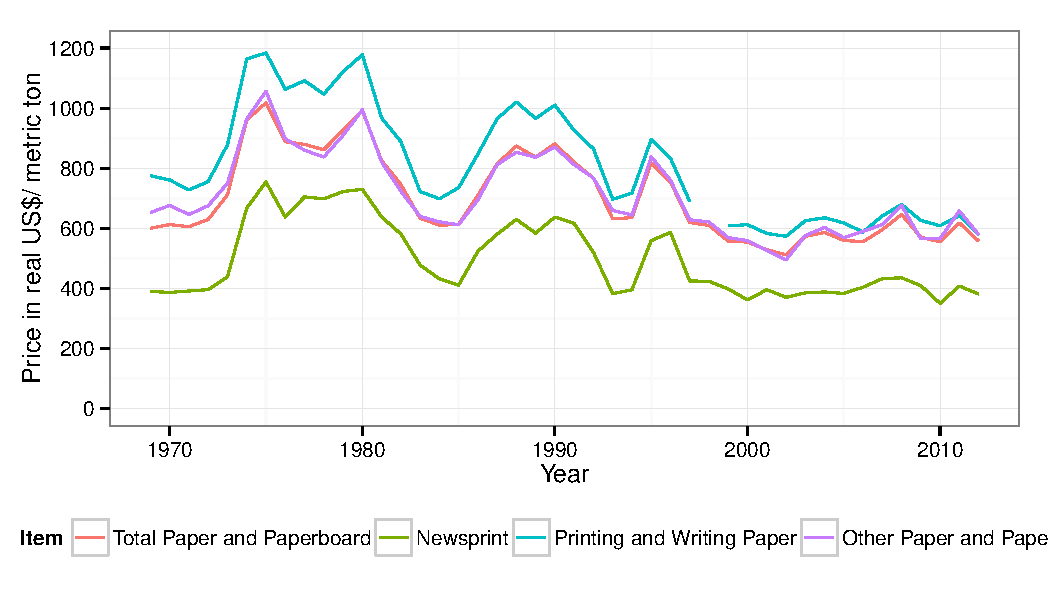
\includegraphics[width=1\linewidth]{figure/PriceEU15Extended} 

}

\caption[Price evolution of paper and paperboard products in EU15 in USD of 1987, source]{Price evolution of paper and paperboard products in EU15 in USD of 1987, source: FAOSTAT and own calculations\label{fig:PriceEU15Extended}}
\end{figure}


\end{knitrout}




\subsection{Prices by Country }
One graph by product, one line for each country. 
Highest and lowest values are highlighted. 
\begin{knitrout}
\definecolor{shadecolor}{rgb}{0.969, 0.969, 0.969}\color{fgcolor}\begin{figure}[h]


{\centering 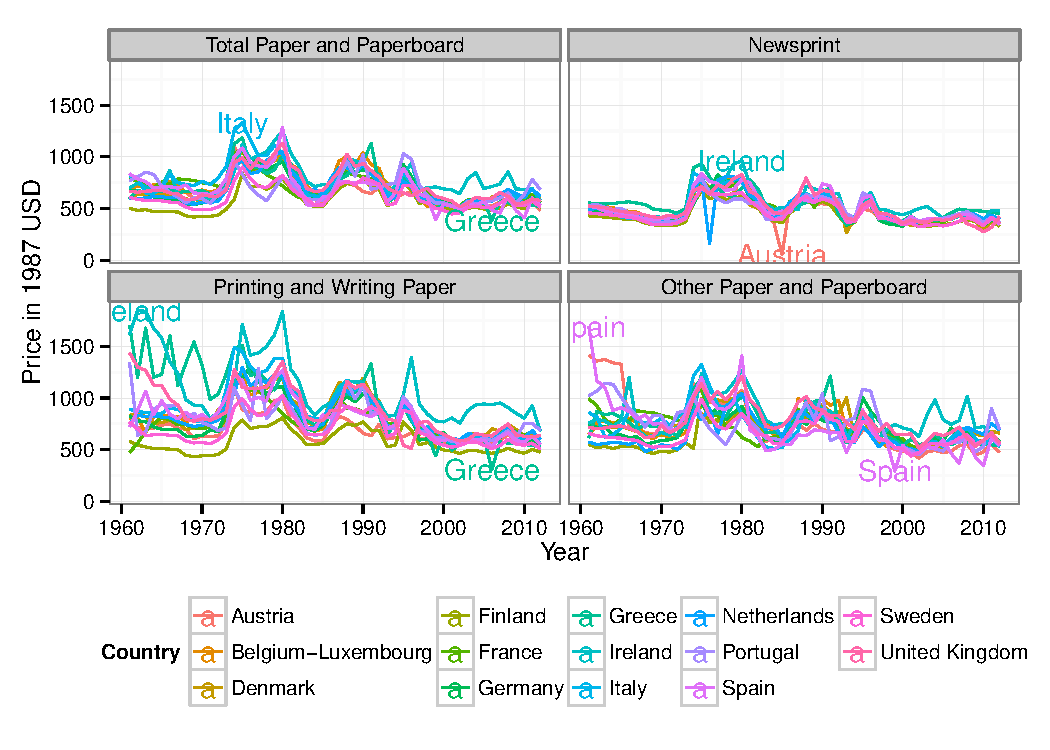
\includegraphics[width=1\linewidth]{figure/PriceByCountry} 

}

\caption[Price by Country, highest and lowest country highlighted]{Price by Country, highest and lowest country highlighted\label{fig:PriceByCountry}}
\end{figure}


\end{knitrout}


\newpage
\subsection{Prices for 4 major countries}
One graph by country one line for each product. Then one graph by product, one line for each country.
\begin{knitrout}
\definecolor{shadecolor}{rgb}{0.969, 0.969, 0.969}\color{fgcolor}\begin{figure}[h]


{\centering 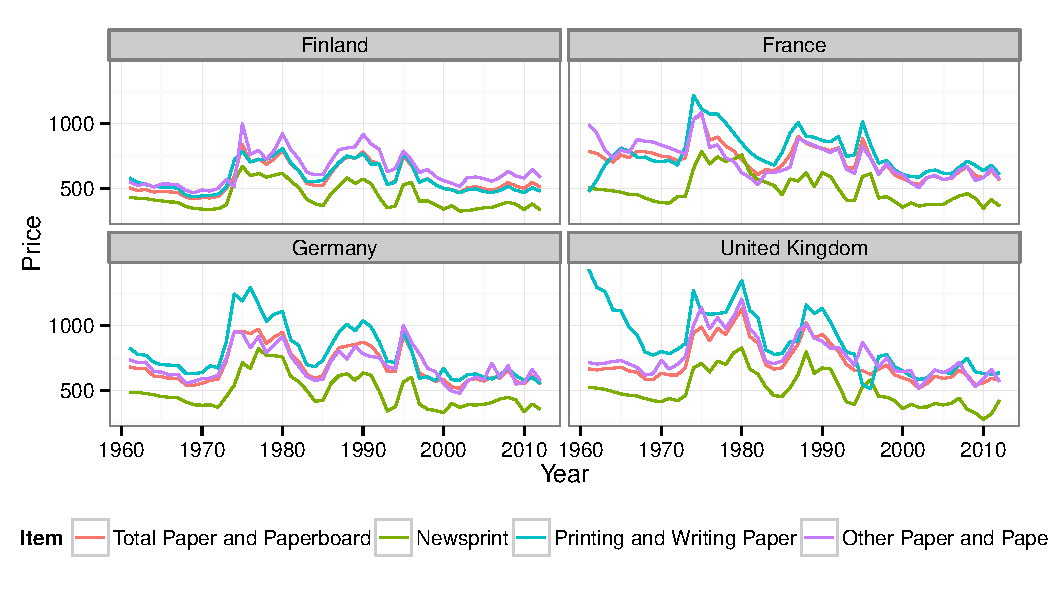
\includegraphics[width=1\linewidth]{figure/Price4MajorCountries1} 

}

\caption[Price evolution of paper and paperboard products in France, Finland, UK and Germany in USD of 1987]{Price evolution of paper and paperboard products in France, Finland, UK and Germany in USD of 1987\label{fig:Price4MajorCountries1}}
\end{figure}

\begin{figure}[h]


{\centering 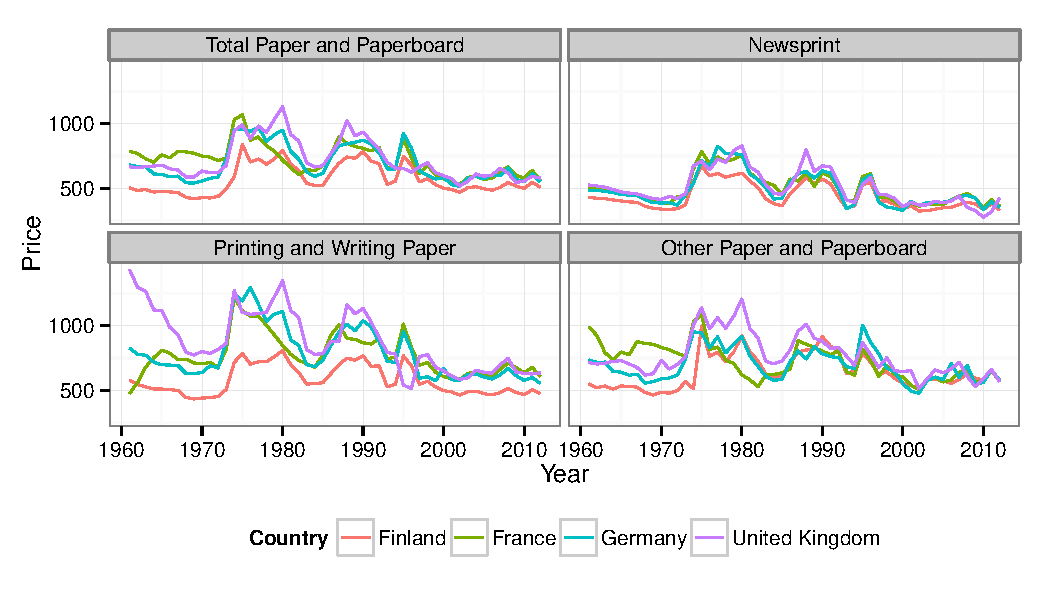
\includegraphics[width=1\linewidth]{figure/Price4MajorCountries2} 

}

\caption[Price evolution of paper and paperboard products in France, Finland, UK and Germany in USD of 1987]{Price evolution of paper and paperboard products in France, Finland, UK and Germany in USD of 1987\label{fig:Price4MajorCountries2}}
\end{figure}


\end{knitrout}



\subsection{Price histograms}
Bar heights correspond to the number of countries in each price range.
\begin{knitrout}
\definecolor{shadecolor}{rgb}{0.969, 0.969, 0.969}\color{fgcolor}\begin{kframe}
\begin{verbatim}
## [1] 1970
\end{verbatim}
\end{kframe}\begin{figure}[h]


{\centering 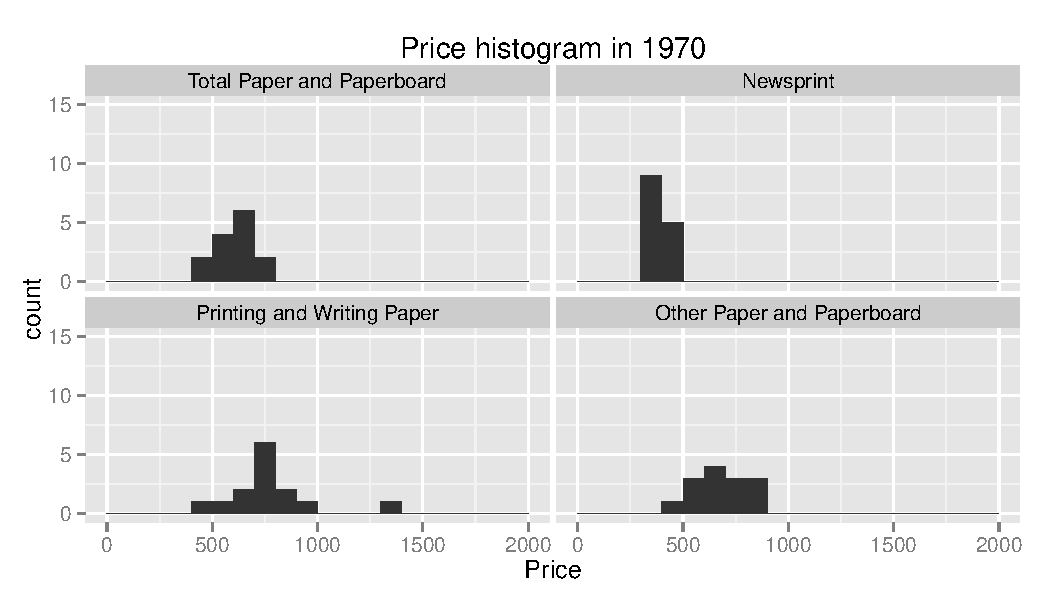
\includegraphics[width=1\linewidth]{figure/PriceHistogram1} 

}

\caption[Price histogram]{Price histogram\label{fig:PriceHistogram1}}
\end{figure}

\begin{kframe}\begin{verbatim}
## [1] 1980
\end{verbatim}
\end{kframe}\begin{figure}[h]


{\centering 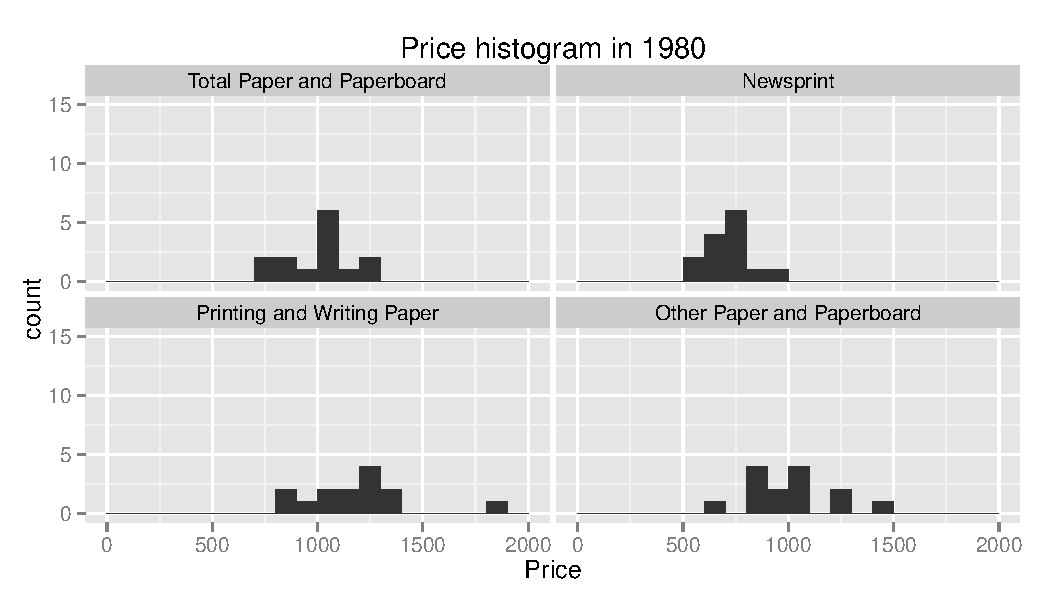
\includegraphics[width=1\linewidth]{figure/PriceHistogram2} 

}

\caption[Price histogram]{Price histogram\label{fig:PriceHistogram2}}
\end{figure}

\begin{kframe}\begin{verbatim}
## [1] 1990
\end{verbatim}
\end{kframe}\begin{figure}[h]


{\centering 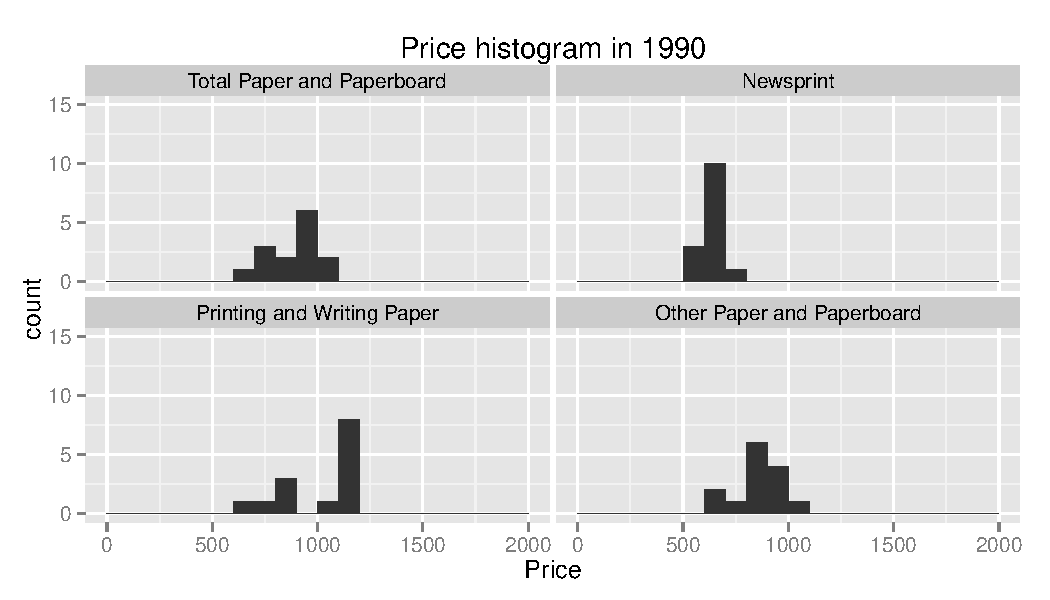
\includegraphics[width=1\linewidth]{figure/PriceHistogram3} 

}

\caption[Price histogram]{Price histogram\label{fig:PriceHistogram3}}
\end{figure}

\begin{kframe}\begin{verbatim}
## [1] 2000
\end{verbatim}
\end{kframe}\begin{figure}[h]


{\centering 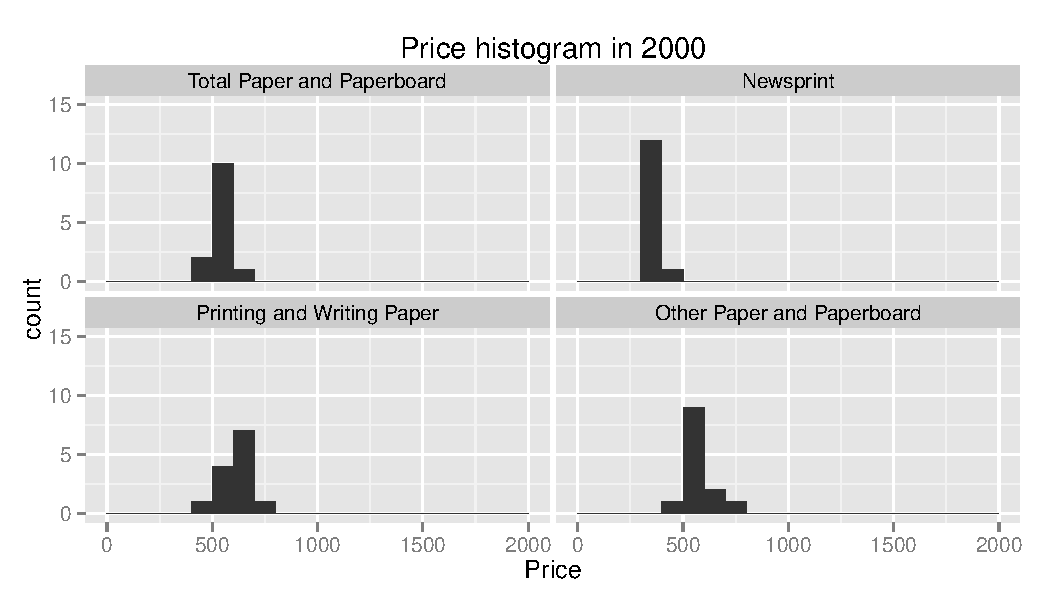
\includegraphics[width=1\linewidth]{figure/PriceHistogram4} 

}

\caption[Price histogram]{Price histogram\label{fig:PriceHistogram4}}
\end{figure}


\end{knitrout}


\end{document}
